\documentclass{article}
\linespread{1.3}
\usepackage[margin=50pt]{geometry}
\usepackage{amsmath, amsthm, amssymb, amsthm, tikz, fancyhdr, graphicx}
\pagestyle{fancy}
\renewcommand{\headrulewidth}{0pt}
\newcommand{\changefont}{\fontsize{15}{15}\selectfont}

\fancypagestyle{firstpageheader}
{
  \fancyhead[R]{\changefont Michael Huang \\ CFRM 420 \\ Homework 3}
}

\begin{document}

\thispagestyle{firstpageheader}

\section*{1.}
{\Large 

% \begin{verbatim}
%   Text enclosed inside \texttt{verbatim}
%   environment 
%   is printed directly 
%   and all \LaTeX{} commands are ignored.
% \end{verbatim}

% \framebox[1.1\width]{\textbf{answer}}

\subsection*{(a)}

We perform this in R using the \texttt{plot} function.

\begin{figure}[h]
  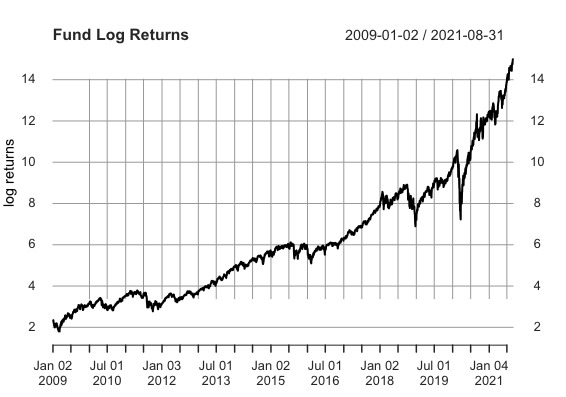
\includegraphics[width=500pt]{hw3_1a.png}}
  \centering
\end{figure}

\subsection*{(b)}

We calculate these using the \texttt{mean}, \texttt{var}, \texttt{skewness} and \texttt{kurtosis}  functions (with the latter adjusted by +3, since it calculates the excess kurtosis): \\
Sample mean: \framebox[1.1\width]{\textbf{0.01320093}} \\ 
Sample variance: \framebox[1.1\width]{\textbf{0.002066732}} \\ 
Sample skewness: \framebox[1.1\width]{\textbf{-0.3651695}} \\ 
Sample kurtosis: \framebox[1.1\width]{\textbf{3.643343}}

\subsection*{(c)}

We take the volatility using the standard deviation, so we use the function \texttt{sd} to determine the volatility of the 3 assets; we take the expected returns by taking the mean, so we use the function \texttt{mean}. We get the following results: \\
Bond: 0.001756121 log returns, 0.004133538 volatility \\
Fund: 0.01320093 log returns, 0.04546132 volatility \\
S\&P 500: 0.011261 log returns 0.04137414 volatility \\ \\ 
From doing this comparison, we see that \framebox[1.1\width]{\textbf{it is not the case}}that assets with higher expected return have higher volatility. In fact, the lowest volatility asset, the bond, has the highest expected log return.

\subsection*{(d)}

We perform said functions in R, and \texttt{plot} as follows. We fit a normal distribution by taking the mean and variance of the distribution and fit as follows. \\


\subsection*{(e)}



}

\section*{2.}
{\Large

\subsection*{(a)}



\subsection*{(b)}



\subsection*{(c)}



}

\end{document}